%%%%%%%%%%%%%%%%%%%%%%%%%%%%%%%%%%%%%%%%%%%%%%%%%%%%%%%%%%%%%%%%%%%%%%%%%%
%
%                         华南理工大学毕业论文模板
%
%   本文件为模板示例，请根据个人需求进行相应修改。
%
%   1. 在使用此模板前，请根据学校提供的论文模板，完成封面（摘要前）的信息，
%      生成 cover.pdf 并上传至 cover 文件夹中，若需要使用匿名盲审版本，可
%      额外上传 cover_blind.pdf 至 cover 文件夹中。
%   2. 有其他包需求的文章，请自行使用 \usepackage
%   3. 通过 documentclass 选项切换学位、版本控制、超链接样式：
%      学位:
%         master:      硕士
%         doctor:      博士
%      版本控制:
%         submission:  系统最终提交版本，必须提供 cover/cover.pdf 封面
%         blindreview: 匿名盲审版本，建议额外提供 cover/cover_blind.pdf 封
%                      面，论文一般需要重命名为 10561_学号_LW.pdf
%         maincontent: 论文正文版本，只含绪论、正文、结论，一般用于查重，
%                      论文一般需要重命名为 10561_学号_ZT.pdf
%      超链接样式:
%         manuscript: 手稿样式，适合在线阅读
%         final:      提交样式，适合打印，去除超链接颜色和边框
%   4. 专为 Bash 用户设计的一键论文生成脚本 generate 已提供，位于 scripts
%      文件夹中，能同时提供用于提交、盲审、查重的三种版本的 PDF 文件，并且
%      提供包含摘要的 TXT 文件，方便在线提交系统。学号和学校 ID 需要在
%      generate 脚本中进行设置，生成的 PDF 文件会保存在 output 文件夹中。
%
%%%%%%%%%%%%%%%%%%%%%%%%%%%%%%%%%%%%%%%%%%%%%%%%%%%%%%%%%%%%%%%%%%%%%%%%%%

\documentclass[unicode,master,submission,final]{scutthesis}

%%%%%%%%%%%%%%%%%%%%%%%%%%%%%%%%%%%%%%%%%%%%%%
% TeX 功能包设置
%%%%%%%%%%%%%%%%%%%%%%%%%%%%%%%%%%%%%%%%%%%%%%
\usepackage{fix-cm}
\usepackage{anyfontsize}
\usepackage{fontspec,color,array,longtable,graphicx}
\usepackage{bytefield}
\usepackage{fancyhdr}
\usepackage{xunicode}
\usepackage[backend=biber,style=gb7714-2015,gbalign=gb7714-2015,gbpub=false,gbnamefmt=lowercase]{biblatex}
% 参考文献导入
\addbibresource{article.bib}

%%%%%%%%%%%%%%%%%%%%%%%%%%%%%%%%%%%%%%%%%%%%%%
% 页眉页脚设置
%%%%%%%%%%%%%%%%%%%%%%%%%%%%%%%%%%%%%%%%%%%%%%
\pagestyle{fancy}
\fancyfoot[C]{\headfont\thepage}
\renewcommand{\chaptermark}[1]{\markboth{\chaptername\ #1}{}}
\renewcommand{\sectionmark}[1]{\markright{\thesection\ #1}}
\fancyhead[RE]{}
\fancyhead[RO]{}
\fancyhead[LE]{}
\fancyhead[LO]{}
\fancyhead[CO]{\headfont{\leftmark}}
\fancyhead[CE]{\headfont{\thesissubject}}%
\renewcommand{\headrulewidth}{1.5pt}
\renewcommand{\footrulewidth}{0pt}

%%%%%%%%%%%%%%%%%%%%%%%%%%%%%%%%%%%%%%%%%%%%%%
% 封面设置
%%%%%%%%%%%%%%%%%%%%%%%%%%%%%%%%%%%%%%%%%%%%%%
\usepackage[unicode=true,bookmarks=true,bookmarksnumbered=true,bookmarksopen=false,breaklinks=false,pdfborder={0 0 1},backref=false,colorlinks=true]{hyperref}

\thesishypersetup

\begin{document}

\maketitle
\frontmatter
\ifmaincontent\else

%%%%%%%%%%%%%%%%%%%%%%%%%%%%%%%%%%%%%%%%%%%%%%
% 摘要
%%%%%%%%%%%%%%%%%%%%%%%%%%%%%%%%%%%%%%%%%%%%%%
% 中文摘要
\chapter{摘\texorpdfstring{\quad}{}要}

本文为毕业论文模板正文示例，用于展示常见结构与排版方式。请在此处概述研究背景、研究问题、方法、结果与结论，建议按照“背景-方法-结果-结论”的逻辑组织摘要内容。

本文的主要工作可概括为：

（1）工作一：概述方法或系统

（2）工作二：概述实验或验证

（3）工作三：概述结论或贡献

\keywordsCN{关键词1；关键词2；关键词3；关键词4}

% 英文摘要
\chapter{Abstract}

This document is a thesis template example that demonstrates structure and formatting. Replace this paragraph with your study background, problem statement, methods, results, and conclusions.

The main contributions include:

(1) [Contribution 1: method or system]

(2) [Contribution 2: experiments or validation]

(3) [Contribution 3: conclusions or impact]

\keywordsEN{Keyword1; Keyword2; Keyword3; Keyword4}

%%%%%%%%%%%%%%%%%%%%%%%%%%%%%%%%%%%%%%%%%%%%%%%%
% 目录
%%%%%%%%%%%%%%%%%%%%%%%%%%%%%%%%%%%%%%%%%%%%%%%%
%\cleardoublepage % pdfbookmark可能需要这一条才能正常工作
\pdfbookmark{\contentsname}{toc} %为目录添加pdf文件书签
\tableofcontents
\fi

\mainmatter

% 正文部分页眉页脚微调（每章第一页均设置页眉页脚）
\fancypagestyle{plain}{\pagestyle{fancy}}
\pagestyle{fancy}

%%%%%%%%%%%%%%%%%%%%%%%%%%%%%%%%%%%%%%%%%%%%%%
% 第一章：绪论
%%%%%%%%%%%%%%%%%%%%%%%%%%%%%%%%%%%%%%%%%%%%%%
\chapter{绪论}

\section{课题研究背景和意义}

本节用于交代研究的现实背景与学术价值。建议按“行业趋势—关键问题—研究空白”的结构展开，并回答以下问题：为什么要做、要解决什么、解决了有什么价值。示例写法如下：

随着行业的发展，出现了...趋势。然而在...中仍存在...与...，例如准确性不足/成本过高/效率受限等。现有研究多聚焦于...技术路线并取得一定进展，但在...限制条件下仍存在不足。基于此，本文围绕研究主题展开研究，期望在目标指标与应用价值方面取得改进。

\section{研究现状}

本节用于综述与本文主题相关的研究进展。建议按“方法类别—关键假设—优缺点—适用场景”组织，并给出代表性文献\cite{sample1,sample2,sample3}。可采用如下模板：

（1）方法类别A：主要思路为（简述），优势在（优势点），不足在（限制条件）。

（2）方法类别B：主要思路为（简述），适用于（场景），但在（问题）上仍需改进。

（3）方法类别C：侧重（维度），常与技术/模型结合，面临（挑战）。

综合来看，现有研究为本文提供了基础/工具，但在本文关注点方面仍存在研究空间。

\section{本文研究内容}

\subsection{课题来源}

请在此处说明课题来源或项目背景，例如项目名称/资助来源/实际需求单位。若不便公开，可写为“本课题源于实际工程需求/合作项目/公开数据任务”。

\subsection{论文研究内容与组织结构}

本文主要研究内容可概括为：

（1）研究内容一：方法/模型/系统（可替换）。

（2）研究内容二：实验/验证/对比（可替换）。

（3）研究内容三：应用/扩展/总结（可替换）。

论文结构安排如下：第一章为绪论，介绍研究背景与意义及相关工作；第二章给出基础理论与概念；第三章描述方法与实现；第四章给出实验设计与结果分析；第五章介绍系统实现或应用示例；最后在总结与展望中概括工作并提出未来方向。

%%%%%%%%%%%%%%%%%%%%%%%%%%%%%%%%%%%%%%%%%%%%%%
% 第二章：相关工作与基础理论
%%%%%%%%%%%%%%%%%%%%%%%%%%%%%%%%%%%%%%%%%%%%%%
\chapter{相关工作与基础理论}

\section{研究现状综述}

本节进一步聚焦与本文直接相关的核心技术与理论基础。建议按照“问题定义—典型方法—评价指标”的框架展开，并明确本文与现有工作的差异点。例如可从数据驱动/模型驱动、监督/无监督或集中式/分布式等维度进行比较，并指出本文将重点改进的环节。

必要时可给出一张对比表，列出代表性工作、关键假设、数据规模与结果指标，便于读者快速理解研究脉络。

\section{基本概念与符号}

本节用于统一符号与基本定义。建议先给出问题变量、参数与输出的符号表，再给出关键假设或约束。

示例：记输入为 $x$，参数为 $\theta$，输出为 $y$，则有
\begin{equation}
    y = f(x; \theta)
\end{equation}
其中 $f(\cdot)$ 表示模型/映射/系统，$\theta$ 为参数含义。若存在约束条件，可写为
\begin{equation}
    x \in \mathcal X,\quad \theta \in \Theta
\end{equation}
请根据实际研究内容补充符号定义、假设条件与约束说明。

%%%%%%%%%%%%%%%%%%%%%%%%%%%%%%%%%%%%%%%%%%%%%%
% 第三章：方法与实现
%%%%%%%%%%%%%%%%%%%%%%%%%%%%%%%%%%%%%%%%%%%%%%
\chapter{方法与实现}

\section{总体方案}

本章描述方法的总体流程与模块划分。典型步骤可包括：数据获取、特征提取、模型构建、优化求解与结果输出。

\begin{enumerate}
    \item 数据准备与预处理。
    \item 关键方法或模型构建。
    \item 参数估计与结果生成。
    \item 误差分析与结果验证。
\end{enumerate}

\section{关键方法示例}

请在此处详细描述核心算法或系统实现细节，可结合公式、伪代码或流程图说明。

\begin{figure}
    \centering
    
\includegraphics[width=\textwidth]{imgs/placeholder.png}
    \caption{方法流程示意图（占位）}
    \label{fig:method-flow}
\end{figure}

如图\ref{fig:method-flow}所示，方法主要包括数据输入、特征提取、模型训练与结果输出四个步骤。请根据实际内容补充细节说明。

\begin{figure}
    \centering
    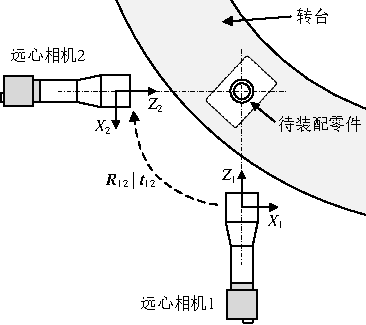
\includegraphics[width=0.5\textwidth]{imgs/chapter3/micro-camera.pdf}
    \caption{微视觉系统相机布局示意图}
    \label{fig:ch3/micro-camera}
\end{figure}

实际书写时，建议将图片按论文章节、按文件夹分类存放，例如 imgs/chapter3/，并且命名规范。如图\ref{fig:ch3/micro-camera}所示，设系统中的两台远心相机分别为相机1和相机2，如图\ref{fig:ch3/micro-camera}所示。其光轴方向分别沿坐标轴$Z_1$和$Z_2$。在理想的正交配置下，两台相机的光轴相互垂直，即相机2的光轴方向与相机1的某一成像平面轴（例如$X_1$轴）平行。不失一般性，假设两台相机之间的相对位姿关系可由旋转矩阵$\bm R_{12}$和平移向量$\bm t_{12}$描述。

此外，还可以使用定理环境来描述方法中的重要结论，例如：

\begin{proposition}\label{ch2/prop:1}
    设函数 $f$ 满足条件 $C$，则在条件 $D$ 下，结论 $E$ 成立。
\end{proposition}
\begin{proof}
    请在此处给出证明过程，说明关键步骤与逻辑推理。
\end{proof}

\begin{proposition}\label{ch2/prop:2}
    对任意实数 $x$ 与 $y$，都有不等式 $x^2+y^2\ge 2xy$。
\end{proposition}
\begin{proof}
    由平方非负性可得
    \begin{equation}
        (x-y)^2\ge 0
    \end{equation}
    展开得
    \begin{equation}
        x^2-2xy+y^2\ge 0
    \end{equation}
    整理即得
    \begin{equation}
        x^2+y^2\ge 2xy
    \end{equation}
\end{proof}

\begin{lemma}\label{ch2/lemma:1}
    设集合 $S$ 满足条件 $M$，则在条件 $N$ 下，性质 $P$ 成立。
\end{lemma}
\begin{proof}
    请在此处给出证明过程，说明关键步骤与逻辑推理。
\end{proof}

\begin{theorem}\label{ch2/theorem:1}
    设算法 $A$ 满足条件 $F$，则在条件 $G$ 下，算法的性能指标 $H$ 达到最优。
\end{theorem}
\begin{proof}
    请在此处给出证明过程，说明关键步骤与逻辑推理。
\end{proof}

%%%%%%%%%%%%%%%%%%%%%%%%%%%%%%%%%%%%%%%%%%%%%%
% 第四章：实验设计与结果
%%%%%%%%%%%%%%%%%%%%%%%%%%%%%%%%%%%%%%%%%%%%%%
\chapter{实验设计与结果}

\section{实验设计}

请在此处说明实验环境、数据来源、评价指标与对比基线，并给出关键参数设置。

\begin{table}[htbp]
    \centering\wuhao
    \caption{实验设置示例（占位）}
    \label{tab:exp-setup}
    \begin{tabular}{lll}
        \toprule
        项目&设置&说明\\
        \midrule
        数据集&数据集名称&规模/来源\\
        指标&指标名称&计算方式\\
        参数&参数名称&取值范围\\
        \bottomrule
    \end{tabular}
\end{table}

\section{结果与讨论}

请在此处给出实验结果并进行分析，说明优势、局限与适用范围，可结合图表与统计指标进行阐释。

%%%%%%%%%%%%%%%%%%%%%%%%%%%%%%%%%%%%%%%%%%%%%%
% 第五章：系统实现与应用示例
%%%%%%%%%%%%%%%%%%%%%%%%%%%%%%%%%%%%%%%%%%%%%%
\chapter{系统实现与应用示例}

\section{系统实现要点}

请在此处描述系统架构、软硬件组成与关键模块接口，强调可复现性与工程可行性。

\section{应用场景与可扩展性}

请在此处说明方法或系统的典型应用场景，讨论在不同数据规模、环境或需求下的可扩展性与改进方向。

%%%%%%%%%%%%%%%%%%%%%%%%%%%%%%%%%%%%%%%%%%%%%%
% 结论
%%%%%%%%%%%%%%%%%%%%%%%%%%%%%%%%%%%%%%%%%%%%%%
\backmatter
\renewcommand{\chaptermark}[1]{\markboth{#1}{}}

\chapter{总结与展望}

\section*{本文总结}\phantomsection
\addcontentsline{toc}{section}{本文总结} % 在目录中添加本文总结

请在此处概括论文的研究目标、主要工作与核心结论，突出创新点与实际价值。

\section*{未来展望}\phantomsection
\addcontentsline{toc}{section}{未来展望}

请在此处给出后续工作方向，例如数据规模扩展、算法优化、系统部署或跨领域应用等。

\ifmaincontent\else
%%%%%%%%%%%%%%%%%%%%%%%%%%%%%%%%%%%%%%%%%%%%%%
% 参考文献
%%%%%%%%%%%%%%%%%%%%%%%%%%%%%%%%%%%%%%%%%%%%%%
% 设置文献著录字号比正文小一号（五号），需要小四号请注释下行.
% \renewcommand*{\bibfont}{\refbodyfont}
\phantomsection
\addcontentsline{toc}{chapter}{参考文献} % 在目录中添加参考文献
\printbibliography

%%%%%%%%%%%%%%%%%%%%%%%%%%%%%%%%%%%%%%%%%%%%%%
% 成果
%%%%%%%%%%%%%%%%%%%%%%%%%%%%%%%%%%%%%%%%%%%%%%
\chapter{攻读\ifmasterdegree{硕士}\else{博士}\fi 学位期间取得的研究成果}
\pubfont
一、已发表（包括已接受待发表）的论文，以及已投稿、或已成文打算投稿、或拟成文投稿的论文情况\underline{\textbf{（只填写与学位论文内容相关的部分）：}}

\blindreview{
% 盲审版（序号、刊物/会议名称、第几作者、年份、文章相关性、收录情况）
\begin{blindachitable}
    \achirow{1&期刊/会议名称&第x作者&20xx&第x章&收录情况}
\end{blindachitable}
}
\submission{
% 提交版（序号、作者、标题、刊物/会议名称、卷期日期页码、文章相关性、收录情况）
\begin{subachitable}
    \achirow{1&作者A, 作者B&论文题目（占位）&期刊名称/级别&20xx, 页码&第x章&收录情况}
\end{subachitable}
}

% 注：在“发表的卷期、年月、页码”栏：
% 1. 如果论文已发表，请填写发表的卷期、年月、页码；
% 2. 如果论文已被接受，填写将要发表的卷期、年月；
% 3. 以上都不是，请据实填写“已投稿”，“拟投稿”。
% 不够请另加页。

二、与学位内容相关的其它成果（包括专利、著作、获奖项目等）

\blindreview{ % 盲审版，仅在 blindreview 环境中生效
    专利：占位，填写专利或其它成果
}
\submission{ % 提交版，在 submission 环境中生效
    专利：占位，填写专利或其它成果
}

\normalsize

%%%%%%%%%%%%%%%%%%%%%%%%%%%%%%%%%%%%%%%%%%%%%%
% 致谢
%%%%%%%%%%%%%%%%%%%%%%%%%%%%%%%%%%%%%%%%%%%%%%
\submission{
\chapter{致\texorpdfstring{\quad}{}谢}

请在此处撰写致谢，感谢导师、同学、家人及资助项目等。内容可根据学校要求调整。

\begin{minipage}[t]{0.945\textwidth}\begin{flushright}
    作者姓名\\
    \today\\         % 自动时间
    % 2026年7月10日\\ % 固定时间
    于华南理工大学
    \par
\end{flushright}\end{minipage}
}
\fi

\end{document}
